\documentclass[10pt]{scrbook} \usepackage{modules/nonstahp_book}
\usepackage{mathspec}

\setmainfont[
	Path = f/,
	BoldFont=pb.ttf,
	ItalicFont=pi.ttf,
	BoldItalicFont=pbi.ttf
		]{p.ttf}
\setsansfont[
	Path = f/,
	BoldFont=pb.ttf,
	ItalicFont=pi.ttf,
	BoldItalicFont=pbi.ttf
		]{p.ttf}
		
\setmathfont(Digits)[Path = f/]{p.ttf}
\setmathfont(Latin)[Path = f/]{pi.ttf}
\setmathfont(Greek)[Path = f/, Uppercase]{p.ttf}
\setmathfont(Greek)[Path = f/, Lowercase]{pi.ttf}

\setmonofont[Path = f/]{pmono.ttf}

%\setCJKmainfont[
%	Path=f/,
%	BoldFont=notoserifb.ttf,
%	ItalicFont=notoserifi.ttf,
%	BoldItalicFont=notoserifbi.ttf
%		]{notoserif.ttf}

 \begin{document}


\task{Треугольник Паскаля}

Этот исследовательский проект состоит из нескольких шагов. Если у вас не получается до конца разобраться в каком-то шаге, пропустите его и изучайте следующий.

\begin{itemize}
\item Найдите сумму чисел в каждой строке треугольника Паскаля.
\item Найдите сумму первого, третьего, пятого, $\ldots$ (и так далее) элемента в какой-нибудь строке треугольника Паскаля. Найдите закономерность.
\item Найдите сумму второго, четвёртого, шестого, $\ldots$ (и так далее) элемента в строке треугольника Паскаля. Найдите закономерность.
\item Найдите сумму квадратов чисел в каждой строке треугольника Паскаля.
\item Выясните, где в треугольнике Паскаля спрятались треугольные числа $T_n = 1+2+\ldots + n$. 
\item А где спрятались пирамидальные числа $P_n = T_1 + T_2 + \ldots + T_n$? А где квадратные числа $S_n = n^2$?
\item Выясните, как связаны числа $1, 11, 11^2, 11^3, 11^4, \ldots$ с треугольником Паскаля.
\item Что будет если взять самый левый элемент в строке треугольника Паскаля, вычесть из него следующий (по--горизонтали), прибавить следующий за ним, затем вычесть следующий, $\ldots$ (и т.д.) до тех пор, пока не кончатся числа в строке? Какое число получится? Найдите закономерность.
\item Ответьте на предыдущий вопрос, если брать не сами элементы треугольника Паскаля, а их квадраты.
\item Выясните, делятся ли все элементы (кроме крайних двух единиц) в строке на номер этой строки (нумерация строк начинается с нуля)? А когда делятся? 
\item Выберите число 1 у края треугольника Паскаля и идите по диагонали вниз. Начните складывать все встречающиеся числа и в какой-нибудь момент остановитесь. Какое число получилось в сумме? А что получится в общем случае?
\item Что получится, если заштриховать все четные числа в треугольнике? Какой будет узор?
\item А если зашриховать все числа, делящиеся на 3?
\item Где спрятались числа Фибоначчи в треугольнике Паскаля?
\item Чему равна сумма чисел в каком-нибудь параллелограмме треугольника Паскаля? Найдите закономерность.
\item Откройте свои собственные закономерности в треугольнике и назовите их в свою честь
\end{itemize}



\task{Задача о разрезании пиццы}

Три разреза через центр круглой пиццы дают шесть кусочков. Если же сделать третий разрез не через центр, то мы получим семь кусочков разной формы и размера. Немного поэкспериментировав, вы убедитесь в том, что наибольшее число кусков, которое вы можете получить с помощью трёх разрезов --- это семь. Но сколько кусочков вы можете получить с помощью большего числа разрезаний?
%\begin{multicols}{2}
\begin{center}
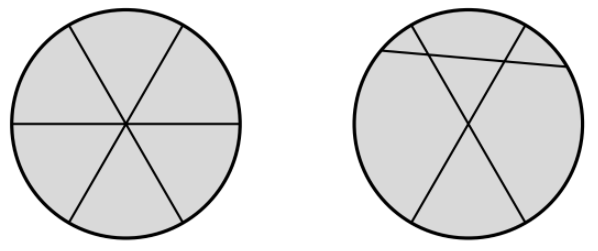
\includegraphics[width=0.85\linewidth]{PizzaC.png}
\end{center}
\begin{itemize}
\item Какое наибольшее число кусочков пиццы вы можете получить с помощью четырёх разрезов?
\item Опишите принцип максимизации для разрезания пиццы. А именно, ответьте на вопрос: как должен проходить новый разрез, чтобы получилось как можно больше кусочков?
\item Пицца Якоба Штейнера имеет бесконечный радиус, а потому о ней можно мыслить просто как о плоскости. Как связан ответ на общую задачу о пицце с ответом на задачу о разрезании пиццы Якоба Штейнера?
\item Через $P_n$ (от слова {\itshape pieces} --- кусочки) обозначим максимальное число кусков, на которое можно разрезать пиццу с помощью $n$ разрезов. Например, $P_1 = 2$ и $P_2 = 4$. Выразите $P_n$ через $P_{n-1}$ и найдите $P_{137}$.
\item Стандартный кусочек пиццы очень похож на треугольник. А как связана задача о разрезании пиццы с треугольными числами?
\item Предположим, что мы получили $P_n$ кусочков пиццы за $n$ разрезаний. Обозначим через $C_n$ (от слова crust --- корка) число тех кусочков пиццы, граница которых не содержит корочки пиццы. Найдите явную формулу для $C_n$.
\item Сложим первые три числа на каждой строчке треугольника Паскаля. Какое число получается?
\item Решите аналогичную {\it задачу о разрезании прямой}. Как вы думаете, а как будет связан ответ на новую задачу с треугольником Паскаля?
\item Решите аналогичную {\it задачу о разрезании арбуза}. Как вы думаете, а как будет связан ответ на новую задачу с треугольником Паскаля? Уже догадались, какой ответы мы получим, если будем разрезать $n$--мерный шар?
\begin{center}
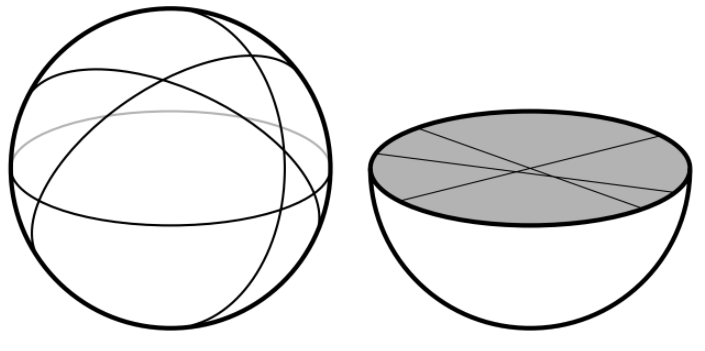
\includegraphics[width=5cm]{PizzaC3.png}
\end{center}
\item Выпишем элементы последовательности $P_n$ в строчку, а под ней запишем её {\it производную последовательность} $\text{Δ} P_n$ (вычитаем из элемента его предыдущий)
\begin{center}
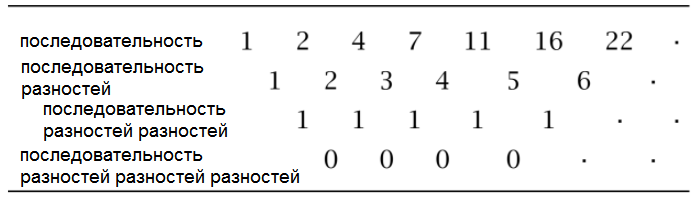
\includegraphics[width=5cm]{PizzaC1.png}
\end{center}
Как видите, четвёртая строка состоит из нулей. Напишите такую же табличку для последовательности каких--нибудь фигурных чисел. 
\begin{center}
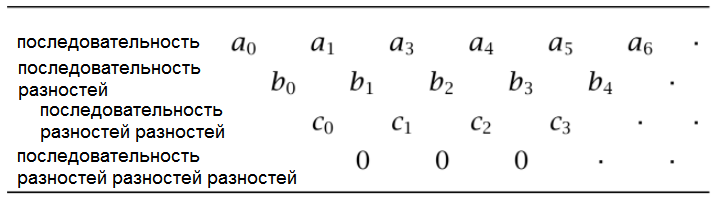
\includegraphics[width=5cm]{PizzaC2.png}
\end{center}
Докажите, что если есть произвольная последовательность $a_n$ обладает тем свойством, что $\text{Δ} c_n = 0$, где $\text{Δ} a_n = b_n$ и $\text{Δ} b_n = c_n$, то\footnote{Через $\binom{n}{k}$ всегда обозначается {\it биномиальный коэффициент} --- элемент в $n$--ой строчке треугольника Паскаля на позиции $k$.}
\begin{align*}
a_n = a_0 \binom{n}{0} + b_0 \binom{n}{1} + c_0 \binom{n}{2}.
\end{align*}
А что можно сказать про последовательности, у которых $c_n = 0$? А $b_n = 0$?
\end{itemize}


\task{Знакомство с простыми числами}

Этот исследовательский проект состоит из нескольких шагов. Если у вас не получается до конца разобраться в каком--то шаге, пропустите его и изучайте следующий. 
%\begin{multicols}{2}
\begin{itemize}
\item Начните писать натуральные числа последовательно вдоль извивающейся линии, как показано на рисунке.
\begin{center}
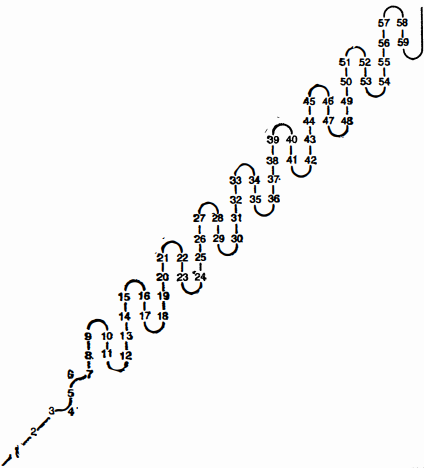
\includegraphics[width=0.85\linewidth]{primes.png}
\end{center}
Найдите на полученной спирали закономерность, связанную с простыми числами, и объясните её.
\item Сколько делителей имеют числа $1, 2, 4, 8, 16, 32, \ldots$? А когда число вида $2^n - 1$ является простым? Составьте таблицу чисел такого вида и найдите закономерность.
\item Выясните, для каких чисел $n$ число $(n-1)!+1$ делится на $n$. Найдите закономерность.
\item Выясните, для каких чисел $n$ число $n^2-1$ делится на 24. Найдите закономерность. 
\item Выясните, для каких чисел $n$ число $n^2+1$ является простым. Найдите закономерность. 
\item Выясните, для каких чисел $n$ число $2^n-2$ делится на $n$. Найдите закономерность. %http://kvant.mccme.ru/1981/09/pochti_prostye_chisla.htm
\item Посмотрим на числа вида $n^2-n$. Получаем $0,2,6,12,20,\ldots$. Все эти числа делятся на два. Посмотрим на числа вида $n^3-n$. Получаем $0, 6, 24, 60, 120, 210, 336, \ldots$. Все эти числа делятся на три! А что дальше? Будут ли числа вида $n^4-n$ делится на четыре? А числа вида $n^5-n$ на пять? Найдите закономерность.
\end{itemize}

\task{Закопеременные представления}

\begin{itemize}
\item Представьте число $1$ в виде произведения нескольких чисел, сумма которых равна нулю.
\item Решите ту же самую задачу для чисел $2,4,6$.
\item Решите эту задачу для числа $3$. Сможете ли вы найти разложение, в котором все числа являются именно целыми, а не рациональными?
\item Исследуйте вопрос представимости для произвольных натуральных чисел.
\end{itemize}

\task{Как же я люблю разрезать!}

\begin{itemize}
\item Возможно ли разрезать на равнобедренные треугольники: а) квадрат\scolon б) прямоугольник? Если --- да, то покажите как.
\item Ответьте на тот же вопрос, если нужно разрезать а) параллелограмм\scolon б) равнобокую трапецию. Если можно, то покажите как.
\item Попытайтесь разрезать фигуры на наименьшее возможное число равнобедренных треугольников.
\item Попробуйте изменить формул фигур из списка выше. Как тогда изменится Ваше разбиение на треугольники? Рассмотрите экстремальные ситуации.
\end{itemize}

\task{Геометрическая миниатюра}

%\begin{multicols}{2}
\begin{itemize}
\item Как вы думаете, какую часть (по площади) составляет треугольник внутри прямоугольника на картинке ниже?
\begin{center}
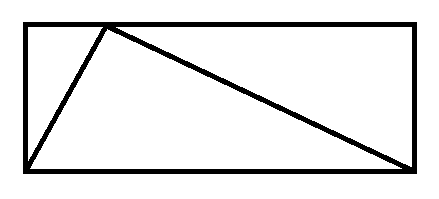
\includegraphics[width=0.7\linewidth]{Area1.png}%1.3
\end{center}
\item А какую часть составляет такой треугольник?
\begin{center}
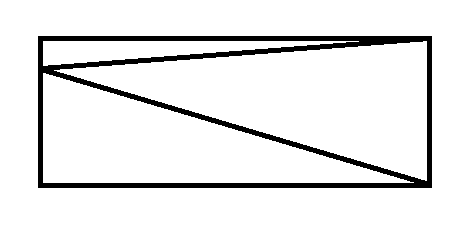
\includegraphics[width=0.7\linewidth]{Area2.png}%1.3
\end{center}
\item Как вы думаете, какую часть (по площади) составляет выделенная область от всего правильного шестиугольника?
\begin{center}
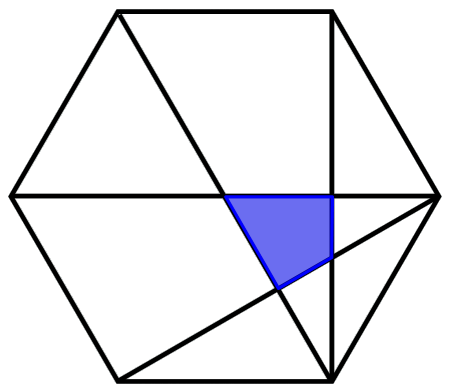
\includegraphics[width=0.7\linewidth]{Area.png}%1.3
\end{center}
\item Выясните, какую часть (по площади) составляет такой треугольник в прямоугольнике
\begin{center}
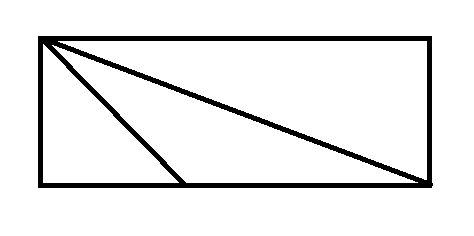
\includegraphics[width=0.7\linewidth]{Area3.png}%1.3
\end{center}
\end{itemize}
%\end{multicols}





\task{Треугольные числа}

%Этот исследовательский проект состоит из нескольких шагов. Если у вас не получается до конца разобраться в каком--то шаге, пропустите его и изучайте следующий.
%\begin{multicols}{2}
\begin{itemize}
\item Можно ли представить число $201745$ в виде суммы двух треугольных чисел?
\item Какие натуральные числа можно представить в виде суммы не более двух треугольных чисел? Найдите закономерность.
\item Какие натуральные числа можно представить в виде суммы не более трёх треугольных чисел? Найдите закономерность.
\item (Золотая теорема). Какие числа можно представить в виде суммы не более $n$ $n$--угольных чисел?
%\item Какие фигуры можно сложить из треугольников, соответствующих треугольным числам?
%\item Что получится, если сложить два последовательных треугольных числа? А что будет, если вычесть из треугольного числа предыдущее треугольное число?
%\item Какие треугольные числа делятся на 3? А какие делятся на 5? А на 7? Есть ли закономерность?
%\item Составьте квадратную табличку, в которой на пересечении $n$--ой строки и $m$--ого столбца стоит сумма треугольных чисел $T_n + T_m$. Все ли натуральные числа встретятся в табличке? А какие не встретятся?
%\item Можно ли представить каждое натуральное число в виде суммы нескольких треугольных чисел?
%\item Можно ли представить каждое натуральное число в виде суммы одного, двух или трёх треугольных чисел? Если нет, то приведите контрпример. Начните с того, что представьте так все числа от 1 до 100.
%\item Ответьте на все вопросы выше для последовательности центрированных треугольных чисел.
\end{itemize}
%\end{multicols}


\task{Шарики в коробках}

Перед вами бесконечный набор коробок, на каждой из которых написано простое число. 
\begin{align*}
2 \quad 3 \quad 5 \quad 7 \quad 11 \quad 13 \quad 17 \quad 19 \quad 23 \quad 29 \quad 31 \quad 37 \quad 41 \quad 43 \quad 47 \quad 53 \quad 59 \quad \ldots
\end{align*}
Вам дали несколько белых шариков и вы решили положить их все в какие--то коробки (в одну коробку можно положить сразу много шириков). 
После этого пришёл эксперт, многозначно посмотрел на вашу расстановку шариков по ящикам и выдал вам число следующим образом: он возвёл число $2$ в степень $\alpha_2$, равную количеству шариков в коробке с надписью $2$, потом возвёл число $3$ в степень $\alpha_3$, равную количеству шариков в коробке с надписью $3$, потом возвёл число $5$ в степень $\alpha_5$, равную количеству шариков в коробке с надписью $5$, и так далее. Затем он умножил все эти числа между собой. Получись число $n = 2^{\alpha_2}\cdot 3^{\alpha_3}\cdot 5^{\alpha_5}\cdot \ldots$.
%\begin{multicols}{2}
\begin{itemize}
\item В коробке $2$ лежит $3$ шарика, а в коробках $3$ и $11$ лежат по одному шарику. Какое число назовёт эксперт?
\item Сколько шариков вам понадобится и куда их нужно положить, чтобы эксперт назвал вам число $6$? А число $12$? А число $21$?
\item В каком случае эксперт назовёт вам простое число? А составное? 
\item Вы расположили шарики в коробках и эксперт назвал число $n$. Что нужно сделать, чтобы он назвал число $np$, где $p$ --- простое число?
\item Известно, что число $n$, которое назвал эксперт, делится на простое число $p$. Что нужно сделать, чтобы эксперт назвал число $n/p$?
\item Вы положили несколько белых шариков в коробки и эксперт назвал Вам число $n$, а потом то же самое происходит с расстановкой чёрных шариков вашего друга --- он получает число $m$. Что нужно сделать, чтобы эксперт назвал число $nm$? А что нужно сделать, чтобы эксперт назвал НОД$(n,m)$? А НОК$(n,m)$? А что можно сказать про расположения белых и чёрных шариков, если числа $n,m$ взаимно просты?
\item Оказалось, что все $m$ шариков положили в одну коробку. Сколько делителей у числа, которое назвал эксперт?
\item Оказалось, что $m$ шариков положили в одну коробку, а $k$ --- в другую. Сколько делителей у числа, которое назвал эксперт?
\item Как определить количество простых делителей числа, которое назовёт эксперт?
\item Правда ли, что можно заставить эксперта назвать любое натуральное число, если правильно подобрать шарики?
% Ваш друг --- несколько чёрных. Затем эксперт назвал Вам и Вашему другу сооветствующие числа $n,m$. Что 
%Что означает тот факт, что $n$ и $m$ взаимно просты?
\end{itemize}
%\end{multicols






\task{Конфигурации точек}

В 2014 г. на Санкт-Петербургской олимпиаде школьников по математике была предложена следующая задача:
\begin{quote}
На двух параллельных прямых отмечено по 40 точек. Их разбивают на 40 пар так, чтобы отрезки, соединяющие точки в одной паре, не пересекались друг с другом. (В частности, конец одного из отрезков не может лежать на другом отрезке). Докажите, что число способов это сделать не превосходит числа $3^{39}$.
\end{quote}
Последовательность, возникающая в этой задаче, обладает богатыми комбинаторными реализациями, их разнообразие просто изумляет. Опишем общую ситуацию: пусть даны две параллельные прямые, на одной отмечено $k$ точек, на другой $n$ точек. 
\begin{center}
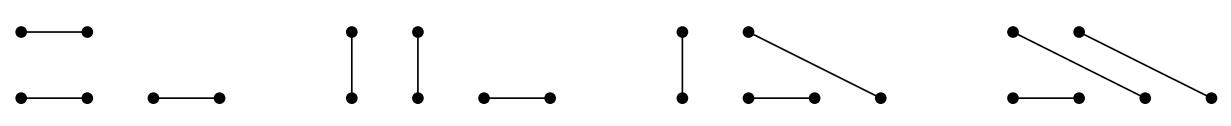
\includegraphics[width=1\linewidth]{Pairs.png}%1.3
\end{center}
Отмеченные точки разбивают на пары так, чтобы отрезки, соединяющие точки в одной паре, не пересекались друг с другом. В частности, конец одного из отрезков не может лежать на другом отрезке. 
\begin{center}
%\begin{figure}[!h]
%\makebox[1 \textwidth][c]{       %centering table
%\resizebox{1 \textwidth}{!}{
\begin{tabular}{c c c c c}
       &       &$[0,0]$&       &     \\
       &$[2,0]$&$[1,1]$&$[0,2]$&     \\
$[4,0]$&$[3,1]$&$[2,2]$&$[1,3]$&$[0,4]$ \\
       &       &$\ldots$&      &
\end{tabular}
%\end{figure}
\end{center}
Полученную картинку будем называть {\it конфигурацией} (точек и отрезков на двух прямых) или {\it разбиением} (точек на пары). Количество разбиений обозначим через $[k,n]$. Например, $[2,4] = 4$, как показывает рисунок выше.
\begin{center}
%\begin{figure}[!h]
%\makebox[1 \textwidth][c]{       %centering table
%\resizebox{1 \textwidth}{!}{
\begin{tabular}{c c c c c c c c c c c c c c}
 &  &  &  & 1&  &  &  & \\% &       &       &$[0,0]$&       &     \\
 &  &  & 1& 1& 1&  &  & \\ % &       &$[2,0]$&$[1,1]$&$[0,2]$&     \\
 &  & 1& 2&  & 2& 1&  & \\% &$[4,0]$&$[3,1]$&$[2,2]$&$[1,3]$&$[0,4]$ \\
 & 1& 3&  &  &  & 3& 1& \\% &       &       &$\ldots$& & \\
1& 4&  &  &  &  &  & 4& 1%&       &       &$\ldots$& &
\end{tabular}
%\end{figure}
\end{center}
%}
%}
Кроме того, если $n+k$ нечётно, то $[k,n] = 0$, а также $[k,n] = 0$, если $n,k < 0$. Если $n$ или $k$ равно нулю, то $[k,n] = 1$ просто по-определению.
\begin{itemize}
\item Заполните треугольник выше и найдите в нём закономерности, аналогичные закономерностям в треугольнике Паскаля.
\item Выясните, какую последовательность образуют суммы элементов в строках треугольника.
\item Правда ли, что в каждой строчке числа $[k,n]$ обязательно возрастают при движении от краёв к центру?
\item Выясните, как выразить $[n,n]$ через суммы квадратов чисел на диагоналях в треугольнике Паскаля.
\end{itemize}


\task{Двойственность}

Как известно, линейная функция задаётся уравнением $y = kx + b$, а графиком линейной функции является прямая. Каждая такая прямая определяется парой чисел $(k,b)$. Построим новую координатную плоскость $(k,b)$, {\it точки} на которой обозначают прямые на исходной координатной плоскости $(x,y)$. 

\begin{itemize}
\item Нарисуйте на плоскости $(x,y)$ какие--нибудь четыре прямые и отметьте их в виде четырёх точек на плоскости $(k,b)$. 
\item Обратно: выберите три точки на плоскости $(k,b)$ и нарисуйте соответствующие три прямые на плоскости $(x,y)$. Что будет, если выбирать точки на $(k,b)$ лежащими на одной вертикальной прямой? А горизонтальной?
\item Рассмотрим на плоскости $(k,b)$ прямую $b=k$. Каждая точка этой прямой задаёт на плоскости $(x,y)$ какую--то прямую, а вся прямая $b=k$ задаёт на плоскости $(x,y)$ набор прямых. Каким свойством обладает этот набор прямых?
\item На координатной плоскости $(k,b)$ проведено три прямые, проходящие через одну точку. Каждая такая прямая изображает некоторый набор прямых на плоскости $(x,y)$. Как эти три набора прямых связаны между собой?
\item Аналогичный вопрос для трёх параллельных прямых на $(k,b)$.
\item Рассмотрим набор всех прямых плоскости $(x,y)$, которые проходят через точку $(0,0)$. Как этот набор изображается на плоскости $(k,b)$? Тот же самый вопрос при замене точки $(0,0)$ на $(m,n)$.
\item Рассмотрим на плоскости $(k,b)$ прямую $b = uk + v$. Какой набор прямых на плоскости $(x,y)$ изображает эта прямая? 
\item Прямые $b = uk + v$ на плоскости $(k,b)$ задают точки на новой плоскости $(u,v)$. Как новая плоскость связана с плоскостью $(x,y)$?
\end{itemize}

\task{Задача Иосифа Флавия}

В книге <<Иудейская война>> Иосифа Флавия есть история о том, как он в составе отряда из 41 иудейского воина был загнан римлянами в пещеру. Предпочитая самоубийство плену, воины решили выстроиться в круг и последовательно убивать каждого третьего из живых, до тех пор пока не останется ни одного человека. Однако Иосиф наряду с одним из своих единомышленников счел подобный конец бессмысленным --- он быстро вычислил спасительные места в порочном круге, на которые поставил себя и своего товарища. И лишь поэтому мы знаем его историю.

В нашем варианте мы начнём с того, что выстроим в круг $n$ человек, пронумерованных числами от $1$ до $n$, и будем исключать каждого {\it второго} из оставшихся до тех пор, пока не уцелеет только один человек. Например, если $n = 10$, то порядок исключения будет такой: 2, 4, 6, 8, 10, 3, 7, 1, 9, так что остаётся номер 5. Убедитесь в этом!
\begin{itemize}
\item Обозначим через $J(n)$ номер последнего уцелевшего человека. Мы только что выяснили, что $J(10) = 5$. Можно было предположить, что $J(n) = n/2$ при чётном $n$. Верно ли это? Начните с $n = 2,3,4,\ldots$.
\item Выпишите табличку, в которой для малых $n$ указаны порядки исключения чисел. Правда ли, что $J(n)$ всегда нечётно? Почему?
\item Пусть $n$ чётно. Выясните, что происходит в тот момент, когда из круга исключается последнее чётное число. Как связаны $J(n)$ и $J(n/2)$?
\item Найдите аналогичную закономерность для нечётного $n$.
\item Пусть $n = 2^m$. Найдите $J(n)$.
\item Выпишите таблицу значений $J(n)$ для $n$ от 1 до 16 и найдите для $J(n)$ явную формулу.
\end{itemize}



\end{document}